\chapter{Computational Study}

This chapter presents our computational study and is structured as follows: 
Section \ref{sec:data} describes the data our experiments are conducted on.
Section \ref{sec:samplesize} examines how different samples sizes used for training affect the test error.
In Section \ref{sec:hpo}, we optimize model hyperparameters and seek to get better intuition when for parameter configuration by analyzing parameters considered for our optimization.
Last but not least, section \ref{sec:noise} demonstrates how noise affects predictive performance of our models.

\section{Data exploration}\label{sec:data}
The available data set is provided by \cite{Hildebrandt2020_EAT} who created a high-dimensional data model with the RMDP instances originally used in \cite{UlmerRMDP}. It comprises 850.469 samples, 23.341 unique customer locations, a delivery fleet of 15 vehicles and 15 unique restaurant locations. The temporal and spatial distribution of the orders is depicted in figure \ref{fig:dists}. 
\begin{figure}[h]
	\centering
	\subfigure[Request arrival time distribution]{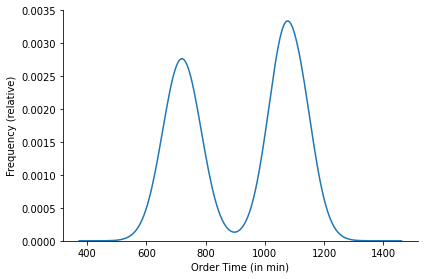
\includegraphics[width=0.49\linewidth]{../Implementation/DataDescription/order_time_dist.png}}
	\subfigure[Spatial distributions]{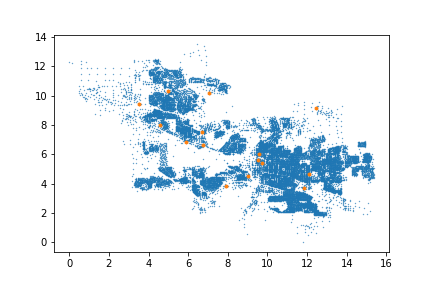
\includegraphics[width=0.49\linewidth]{../Implementation/DataDescription/spatial_dist.png}}
	\caption{Spatial and temporal distributions}
	\label{fig:dists}
\end{figure}

Panel (a) of figure \ref{fig:dists} shows the order behaviour of customers. The x-axis denotes the day time in minutes, the y-axis denotes the relative frequency of incoming customer orders for a given day time on the y-axis. We can observe that the order time behaviour across all customers follows a bimodal gaussian distribution. The order frequency peaks at around 12:00 a.m (roughly 700 minutes of day time) and again around 6.00 p.m (roughly 1100 minutes of day time). This indicates that the probability of an order taking place during lunch or dinner time is relatively high.  
Panel (b) of figure \ref{fig:dists} shows the spatial distribution of customer and restaurant locations. The x-axis depicts the  

\begin{figure}[h]
	\centering
	\subfigure[]{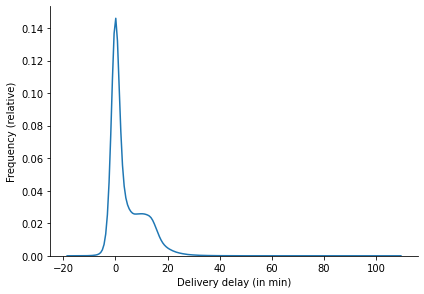
\includegraphics[width=0.49\linewidth]{../Implementation/DataDescription/delivery_delay.png}}
	\subfigure[Temporal distributions]{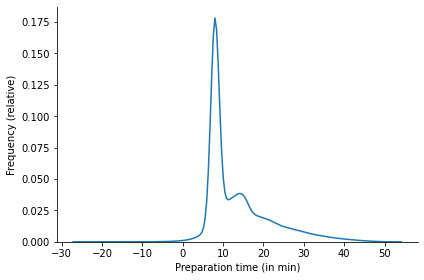
\includegraphics[width=0.49\linewidth]{../Implementation/DataDescription/prep_time.png}}
	\caption{Spatial and temporal distributions}
	\label{fig:prepdelay}
\end{figure}

Panel (a) of figure \ref{fig:predelay} shows the distribution of delivery delay times in minutes for all requests in the data. We notice that deliveries happen on time for 


\section{Experiment: Sample Size tests}\label{sec:samplesize}


\section{Experiment: Hyperparameter Optimization}\label{sec:hpo}
This section presents the hyperparameter optimization (HPO) experiments conducted for GBDTs, RFs, and the neural network architecture presented in section \ref{sec:nn}. 
We use \textit{Optuna} to conduct our HPO experiments, a popular HPO framework presented in \cite{akiba2019optuna}. 
\textit{Optuna} provides a simple implementation design that allows us to analyze evaluated parameters from different points of view. 
The optimizations were conducted on both the crafted data set and the raw data set. 
Concretely, we will proceed as follows: First, we will present the hyperparameters we decided to include in the HPO to then in turn present the optimal hyperparameter values resulting from the experiment and explore the predictive power of different parametrizations. 
For every experiment instance, the hyperparameters will be sampled via the \textbf{C}ovariance \textbf{M}atrix \textbf{A}daption \textbf{E}volution \textbf{S}trategy, or in short \textbf{CMA-ES}. \textit{CMA-ES} follows a simple principle: The probability of samples from previously succesful optimization steps being drawn again is positively correlated to the contribution of those samples to the objective. For further information on \textit{CMA-ES}, the reader is referred to \cite{hansen2016cma}. To speed up the optimization process, we use the \textit{Optuna}-implementation of the \textit{Hyperband Pruner} presented in \cite{li2018hyperband}. 
By that, we hope to get a fine-tuned model that maximizes prediction quality on one hand, and intuition for parametrization on the other.
Secondly, we will use the \textit{optuna} implementation of the \textit{fANOVA} evaluation algorithm presented in \cite{fANOVA} to determine hyperparameter importances. In short, \textit{fANOVA} calculates feature importances by fitting a random forest regression model to the parameter configuration resulting of the HPO and predicting the objective value. For this task, we set the number of estimators to 1000 for every HPO instance.
Thereby, we can assess which parameters impact the model significantly and which parameters are less significant, and especially how the importances differ for the two data sets. 
Lastly, we will examine interdependencies between the evaluated hyperparameters. 
 
\subsection{Tree-based Ensembles}

In this section, we will conduct HPO experiments for the tree-based ensembles. 
We are going to start with the optimization and analysis for GBDT.
For GBDT, we decided to optimize following parameters and set the search spaces for each them as follows:
\begin{description}[font=$\bullet$\scshape\bfseries]
	\item $ \text{learning\_rate} \in [0.01, 0.05] $  in steps of 0.001.
	\item $ \text{max\_depth} \in [5, 100] $ in steps of 0.001.
	\item $ \text{feature\_fraction} \in [0.1, 1.0] $ in steps of 0.01.
	\item $ \text{feature\_fraction\_bynode} \in [0.3, 1.0] $ in steps of 0.01
	\item $ \text{num\_leaves} \in [20, 300] $ in steps of 1
	\item $ \text{min\_child\_samples} \in [10, 400] $ in steps of 1.
	\item $ \text{subsample\_freq} \in [1, 10] $ in steps of 1.
	\item $ \text{subsample} \in [0.3, 1.0] $ in steps of 0.01.
\end{description}
Besides the parameters considered for optimization, we set the number of estimators for one iteration in GBDT to 1000 and enable early stopping with a patience of 50. Our selection of parameter search spaces is the result of trial-and-error since machine learning problems are highly individual and, as we have already demonstrated with our literature review, many different solution approaches are possible. The determination of parameter values respectively parameter search spaces therefore has to happen at least partly in a manual fashion, which is why we regard the trial-and-error heuristic as a suitable approach for the configuration of hyperparameter search spaces. Detailed descriptions of the considered parameters for the \textit{lightgbm}-GBDT implementation can be found under \url{https://lightgbm.readthedocs.io/en/latest/Parameters.html}.

Figures \ref{fig:GBDT_HPO_Raw_ParallelPlot} and \ref{fig:GBDT_HPO_Crafted_ParallelPlot} depict the parameter configurations of each optimization epoch in form of a parallel coordinate plot for GBDT on the raw respectively the crafted data set. Except the vertical gray line one the very left in the plots, each vertical gray axis represents the values ranging within the defined intervall of its corresponding parameter, whereas the very left line represents the axis for the objective values. The lines connecting all the parameter axes represent the parameter configurations of the optimization epochs. The bluer a line, the better the objective value - in our case the mean squared error. 

At first glance, it can be seen directly that the parameter configurations of both plots for good predictive performance are quite similar. For both sets, the mean squared error is minimized when we roughly use two-thirds of the features for each GBDT iteration (feature\_fraction, feature\_fraction\_bynode). Less test error is achieved is more likely when we allow the algorithm to build rather deep trees (max\_depth) while constraining the tree splitting process by specifying a lower bound for the minimal amount of samples a node must contain in order to split it further (min\_child\_samples). We can furthermore see that a better objective value is attained when nearly all samples are used for a GBDT iteration (subsampling) and learning rates range between from 0.03 to 0.05 (learning\_rate).
Training GBDT with optimal parameter configuration using the full available amount of samples results in a mean squared test error of approximately 25.6780 on the raw data, and 27.0852 on the crafted data.
For the optimal parameter configurations for training GBDT on both data sets, the reader is referred to Appendix A.1.
\begin{figure}[h]
	\centering
	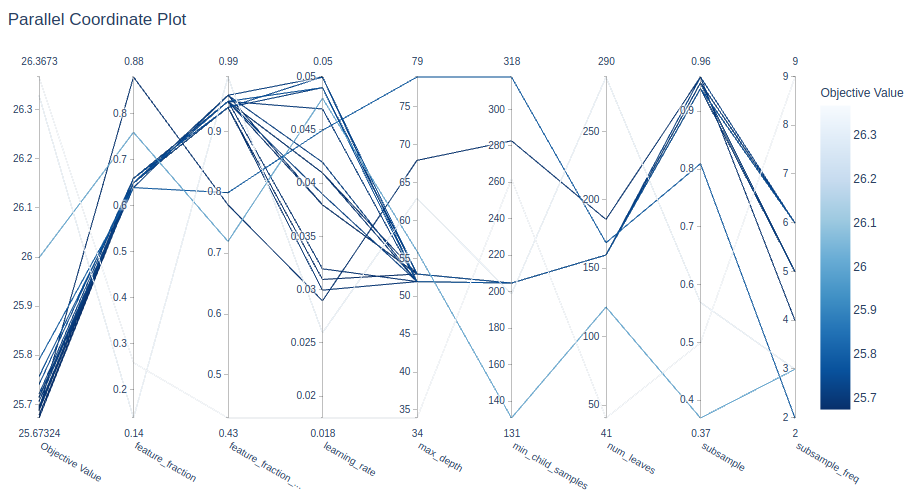
\includegraphics[width=\linewidth]
	{figures/HPO/GBDT_HPO_Raw_ParallelPlot.png}
	\caption{Parallel Coordinate Plot | HPO for GBDT on raw data}
	\label{fig:GBDT_HPO_Raw_ParallelPlot}
\end{figure}
\begin{figure}[h]
	\centering
	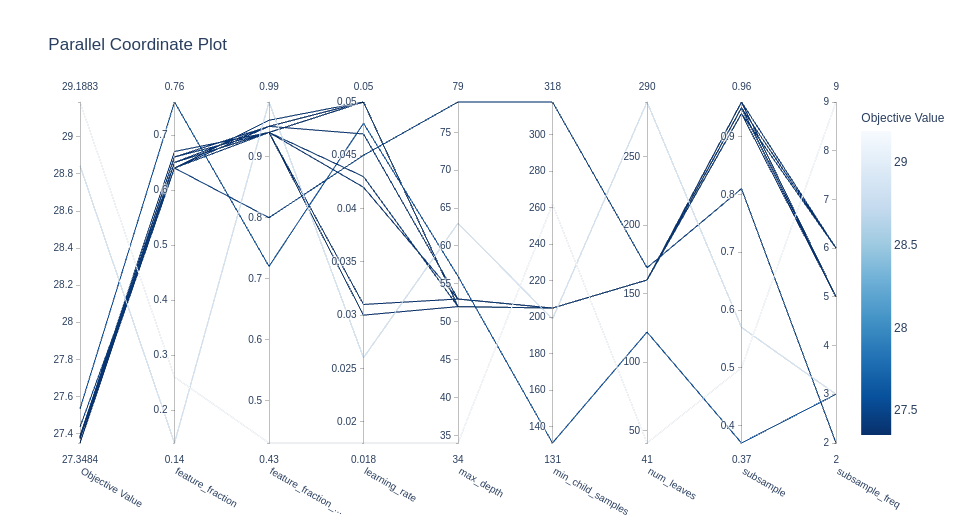
\includegraphics[width=\linewidth]{figures/HPO/GBDT_HPO_Crafted_ParallelPlot.png}
	\caption{Parallel Coordinate Plot | GBDT on crafted data}
	\label{fig:GBDT_HPO_Crafted_ParallelPlot}
\end{figure}

\begin{figure}[h]
	\centering
	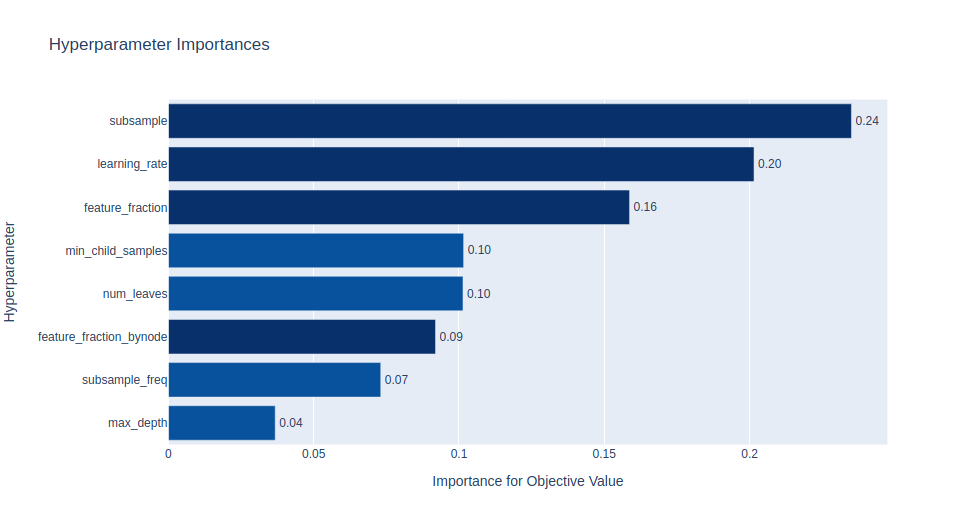
\includegraphics[width=\linewidth]{figures/HPO/GBDT_HPO_Raw_Importances.png}
	\caption{Hyperparameter Importances for GBDT on raw data}
	\label{fig:GBDT_HPO_Raw}
\end{figure}
\begin{figure}[h]
	\centering
	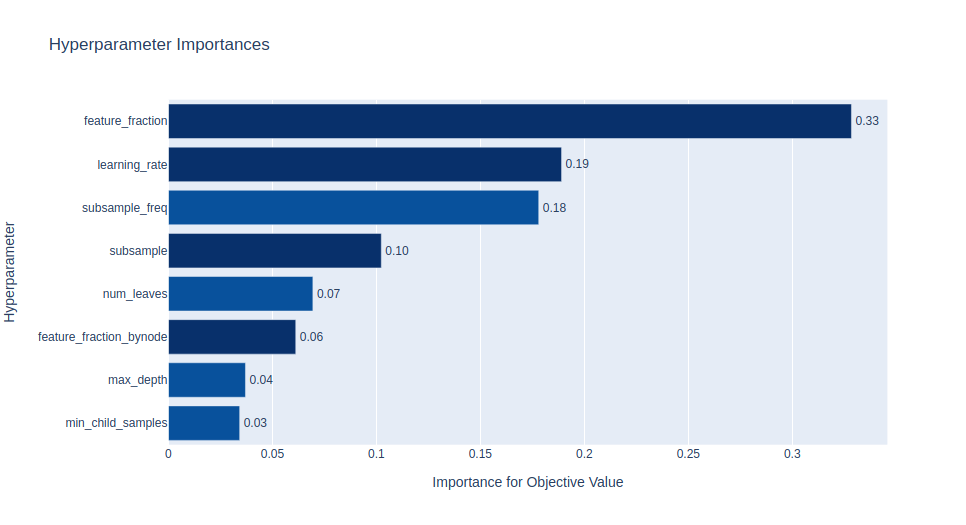
\includegraphics[width=\linewidth]{figures/HPO/GBDT_HPO_Crafted_Importances.png}
	\caption{Hyperparameter Importances for GBDT on crafted data model}
	\label{fig:GBDT_HPO_Crafted}
\end{figure}

\begin{figure}[h]
	\centering
	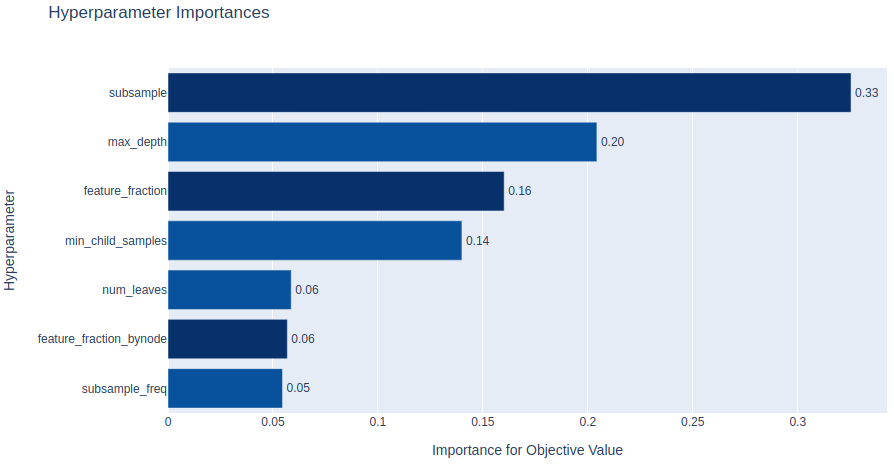
\includegraphics[width=\linewidth]{figures/HPO/RF_HPO_Raw_Importances.png}
	\caption{Hyperparameter Importances for GBDT on crafted data model}
	\label{fig:RF_HPO_Raw_Importances}
\end{figure}
\begin{figure}[h]
	\centering
	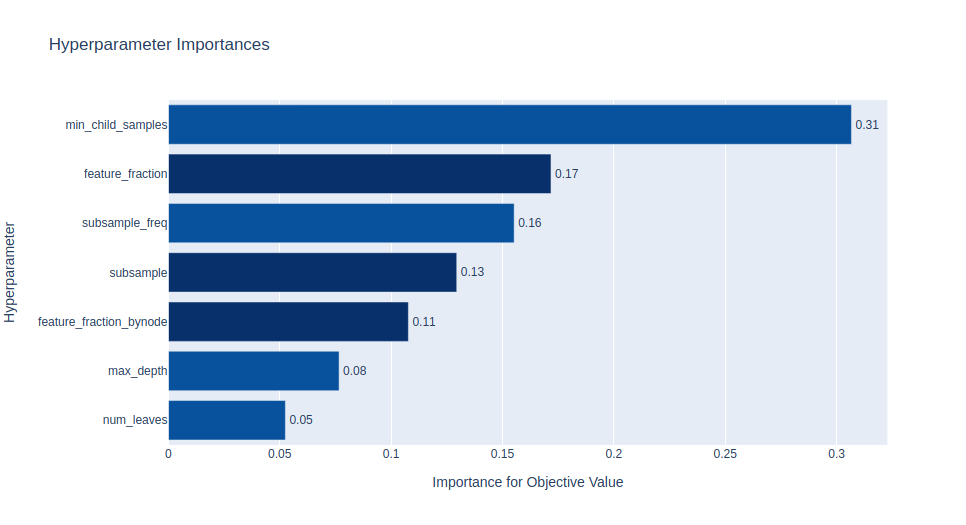
\includegraphics[width=\linewidth]{figures/HPO/RF_HPO_Crafted_Importances.png}
	\caption{Hyperparameter Importances for GBDT on crafted data model}
	\label{fig:RF_HPO_Crafted_Importances}
\end{figure}

%\begin{figure}[h]
%	\centering
%	\subfigure{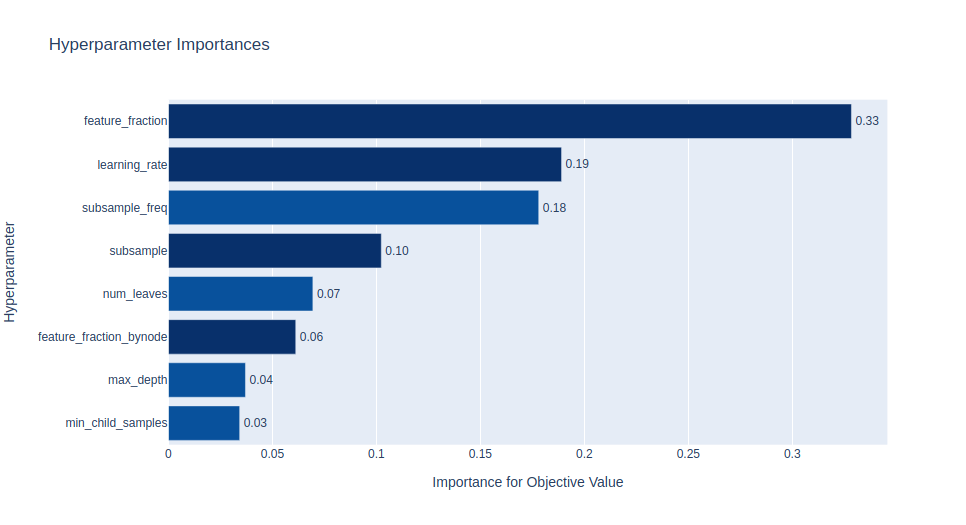
\includegraphics[width=0.49\linewidth]{figures/HPO/GBDT_HPO_Crafted_Importances.png}}
%	\subfigure{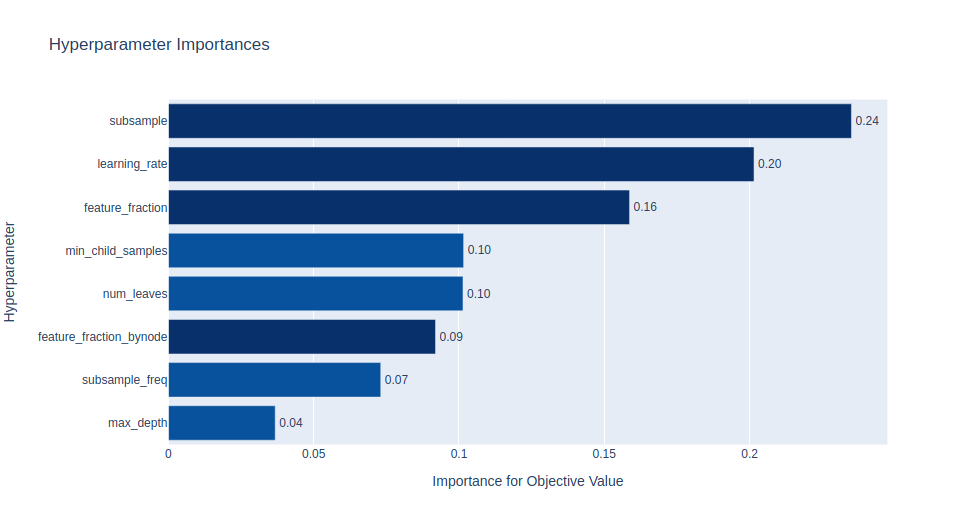
\includegraphics[width=0.49\linewidth]{figures/HPO/GBDT_HPO_Raw_Importances.png}}
%	\caption{Hyperparameter Importances for GBDT on each dataset}
%	\label{fig:GBDT_HPO_Crafted}
%\end{figure}
%\begin{figure}[h]
%	\centering
%	\subfigure{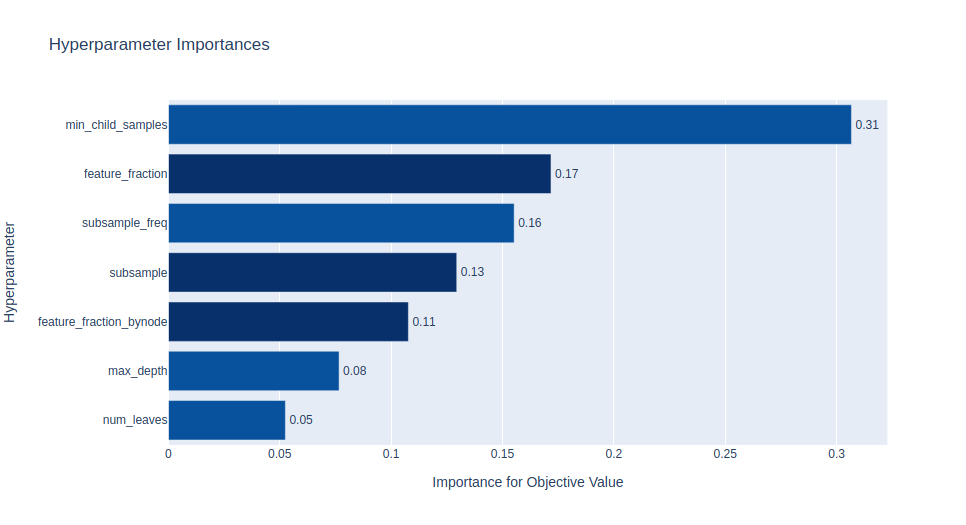
\includegraphics[width=0.49\linewidth]{figures/HPO/RF_HPO_Crafted_Importances.png}}
%	\subfigure{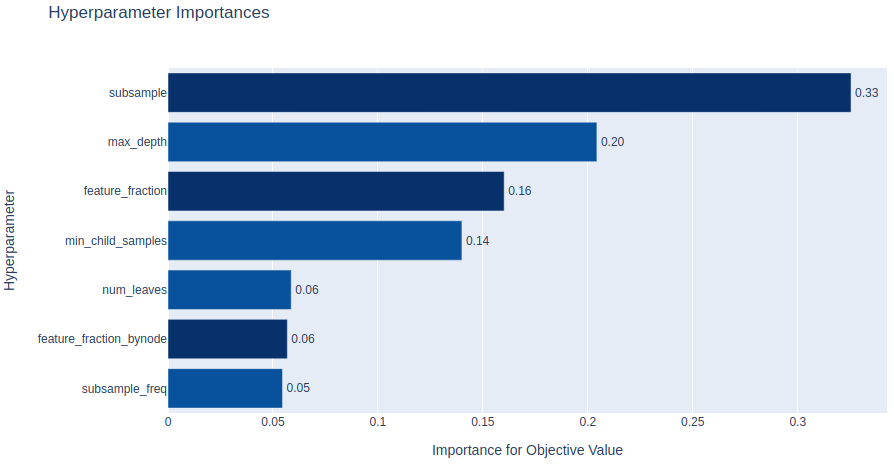
\includegraphics[width=0.49\linewidth]{figures/HPO/RF_HPO_Raw_Importances.png}}
%	\caption{Hyperparameter Importances for RF on each dataset}
%	\label{fig:GBDT_HPO_Crafted}
%\end{figure}

\section{Experiment: Introducing noise}\label{sec:noise}







